\subsection{Modelos significativos y su descripción}

\begin{table}[H]
  \centering
  \small
  \caption{Modelos significativos.}
  \label{tab:modelos}
  \begin{tabularx}{\textwidth}{>{\raggedright\arraybackslash}p{0.24\textwidth}>{\raggedright\arraybackslash}p{0.17\textwidth}>{\raggedright\arraybackslash}X>{\raggedright\arraybackslash}X}
    \toprule
    Modelo & Entrada & Qué se entrena & Qué se elige con validación cruzada interna \\
    \midrule
    Modelo 1: CNN propia & Foto original $384\times288$ & Toda la red (4 bloques de 32/64/128/256 filtros) & Época de paro \\
    \addlinespace
    Modelo 2: ConvNeXt-Tiny preentrenado congelado & Foto sin fondo $384\times288$ & Solo la cabeza & 1 receta de 25 (ridge o MLP $\times$ estiramiento) \\
    \addlinespace
    Modelo 3: EVA02 con ajuste fino (no terminado) & Foto sin fondo $392\times294$ & Toda la red, 5 semillas & Tasa de aprendizaje, época de paro y estiramiento de la salida \\
    \addlinespace
    Modelo 4: ResNet-50 entrenada con fotos de vacas, congelada & Foto sin fondo $512\times384$ & Solo la cabeza & 1 receta de 25 \\
    \addlinespace
    Modelo 5: clasificación del BCS con valor esperado & Características de la red de vacas & Clasificador por cuartos de punto; la salida es el valor esperado & Ajustes del clasificador \\
    \addlinespace
    Salida redondeada a 0.25 & Salida del modelo & Nada (regla fija) & Nada: redondeo a 0.25 dentro del rango del entrenamiento \\
    \addlinespace
    Lectura de la salida del Modelo 5 & Probabilidades del Modelo 5 & Nada & Una de tres lecturas (valor esperado redondeado a 0.25, valor esperado continuo o clase más probable) \\
    \bottomrule
  \end{tabularx}
\end{table}

\begin{itemize}
  \item CNN propia: una red pequeña que mira la foto completa y aprende desde cero. Es el modelo base.
  \item ConvNeXt-Tiny preentrenado congelado: una red grande, ya entrenada con imágenes generales, que no se modifica; convierte cada foto en un resumen de 768 números y una fórmula sencilla traduce ese resumen a BCS.
  \item EVA02 con ajuste fino: la misma idea, pero la red sí se reajusta con nuestras fotos, varias veces con distinto azar. Se lanzó, pero no se terminó por su costo de cómputo.
  \item ResNet-50 entrenada con fotos de vacas, congelada: como el Modelo 2, pero la red que hace el resumen fue entrenada específicamente con fotos de anca de vacas lecheras.
  \item Clasificación del BCS con valor esperado: en lugar de predecir un número directamente, estima la probabilidad de cada cuarto de punto y entrega el promedio ponderado.
  \item Salida redondeada a 0.25: la calificación final se entrega en cuartos de punto, como la reporta el experto.
  \item Lectura de la salida del Modelo 5: la forma de convertir sus probabilidades en un BCS se elige dentro de la validación de cada pliegue, sin mirar las vacas de prueba.
\end{itemize}

\begin{figure}[H]
  \centering
  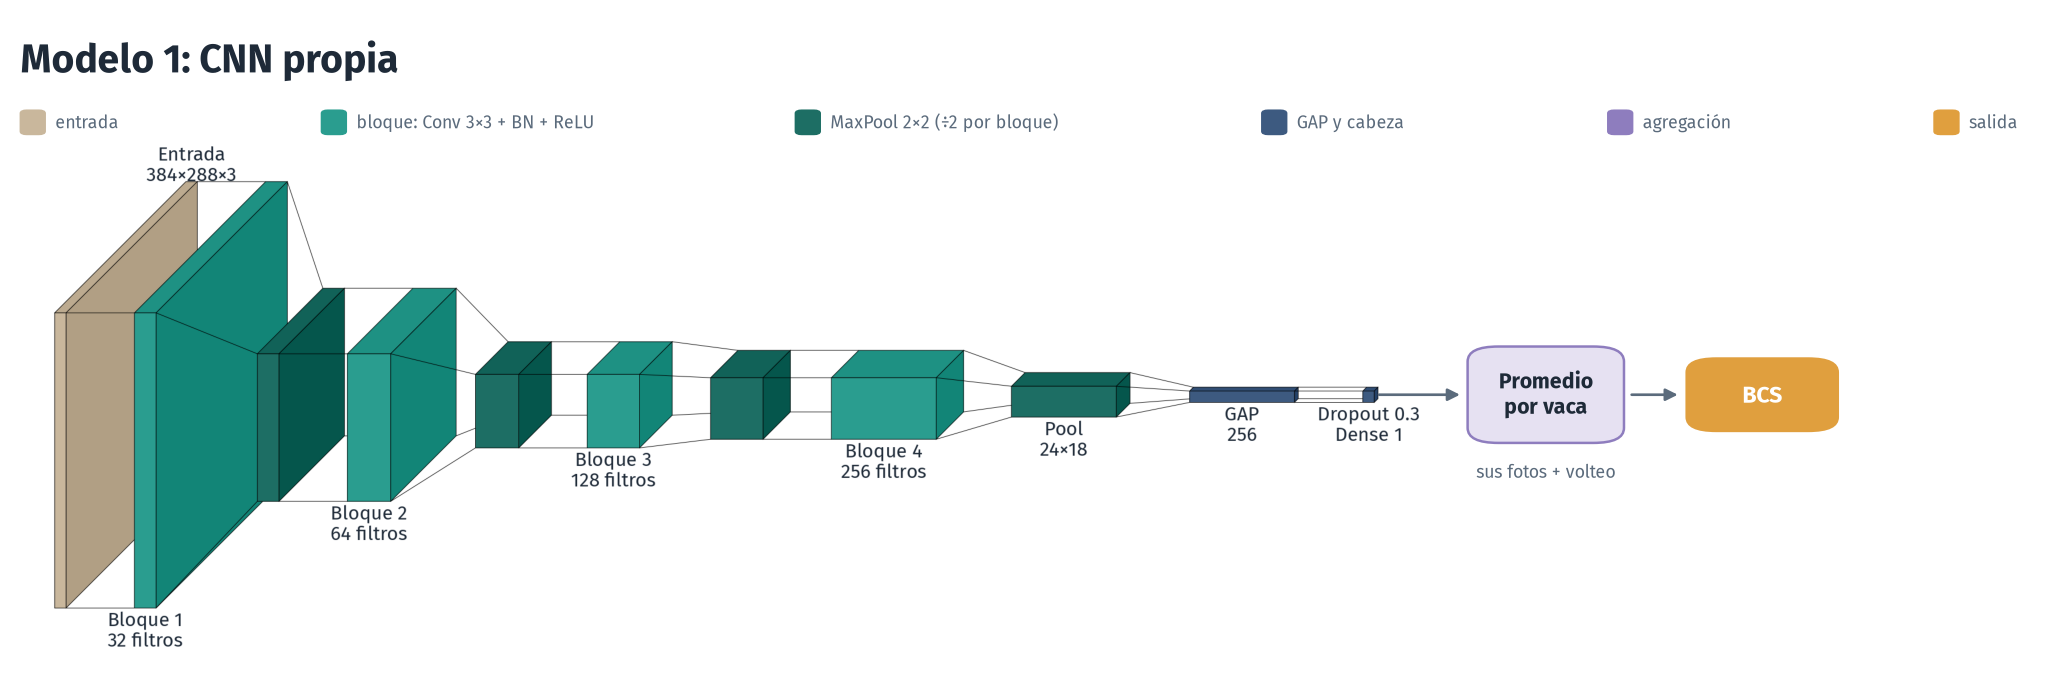
\includegraphics[width=\textwidth]{figures/modelo1}
  \caption{Arquitectura del Modelo 1 (CNN propia).}
  \label{fig:modelo1}
\end{figure}

\begin{figure}[H]
  \centering
  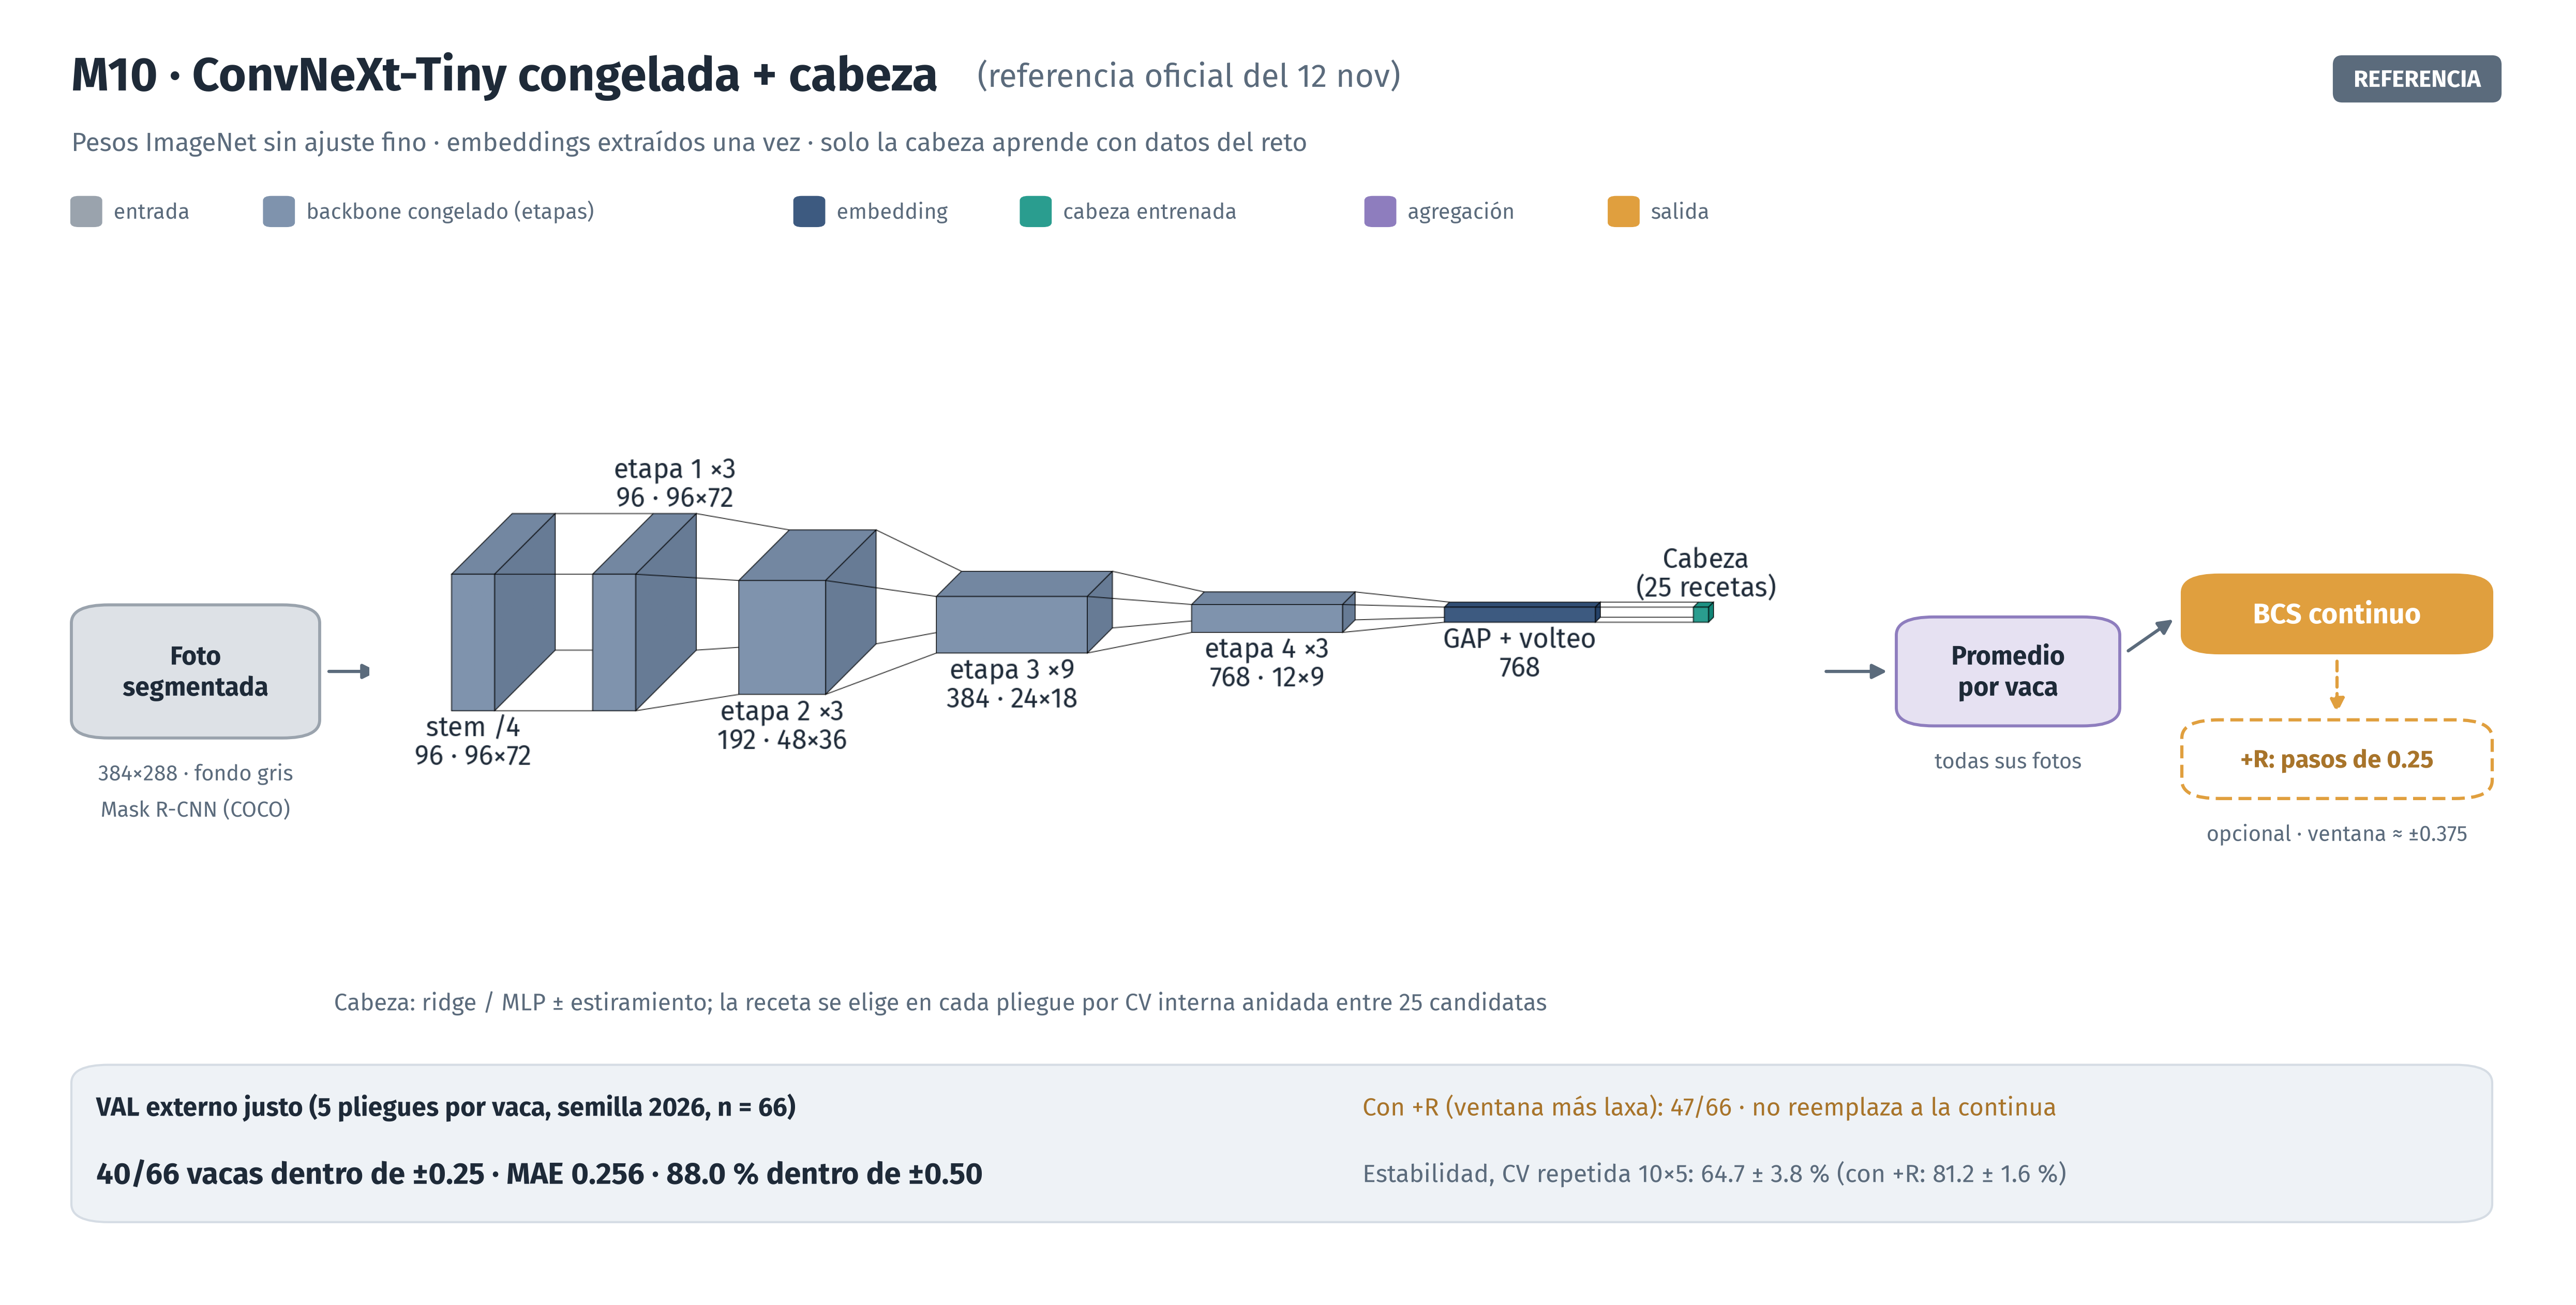
\includegraphics[width=\textwidth]{figures/modelo2}
  \caption{Arquitectura del Modelo 2 (ConvNeXt-Tiny congelado).}
  \label{fig:modelo2}
\end{figure}

\begin{figure}[H]
  \centering
  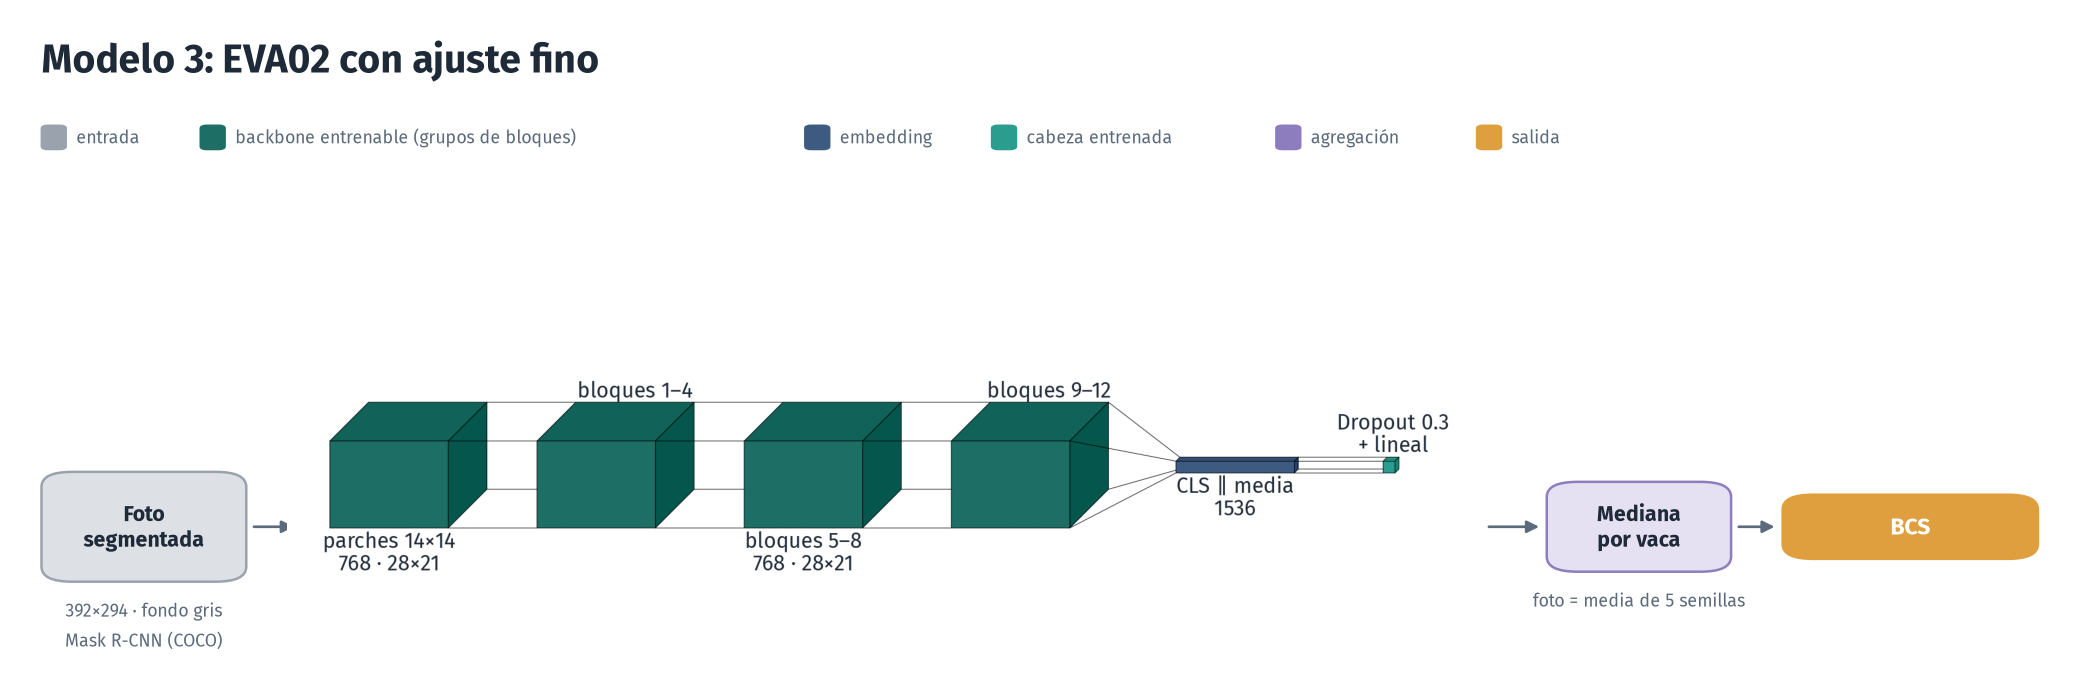
\includegraphics[width=\textwidth]{figures/modelo3}
  \caption{Arquitectura del Modelo 3 (EVA02 con ajuste fino).}
  \label{fig:modelo3}
\end{figure}

\begin{figure}[H]
  \centering
  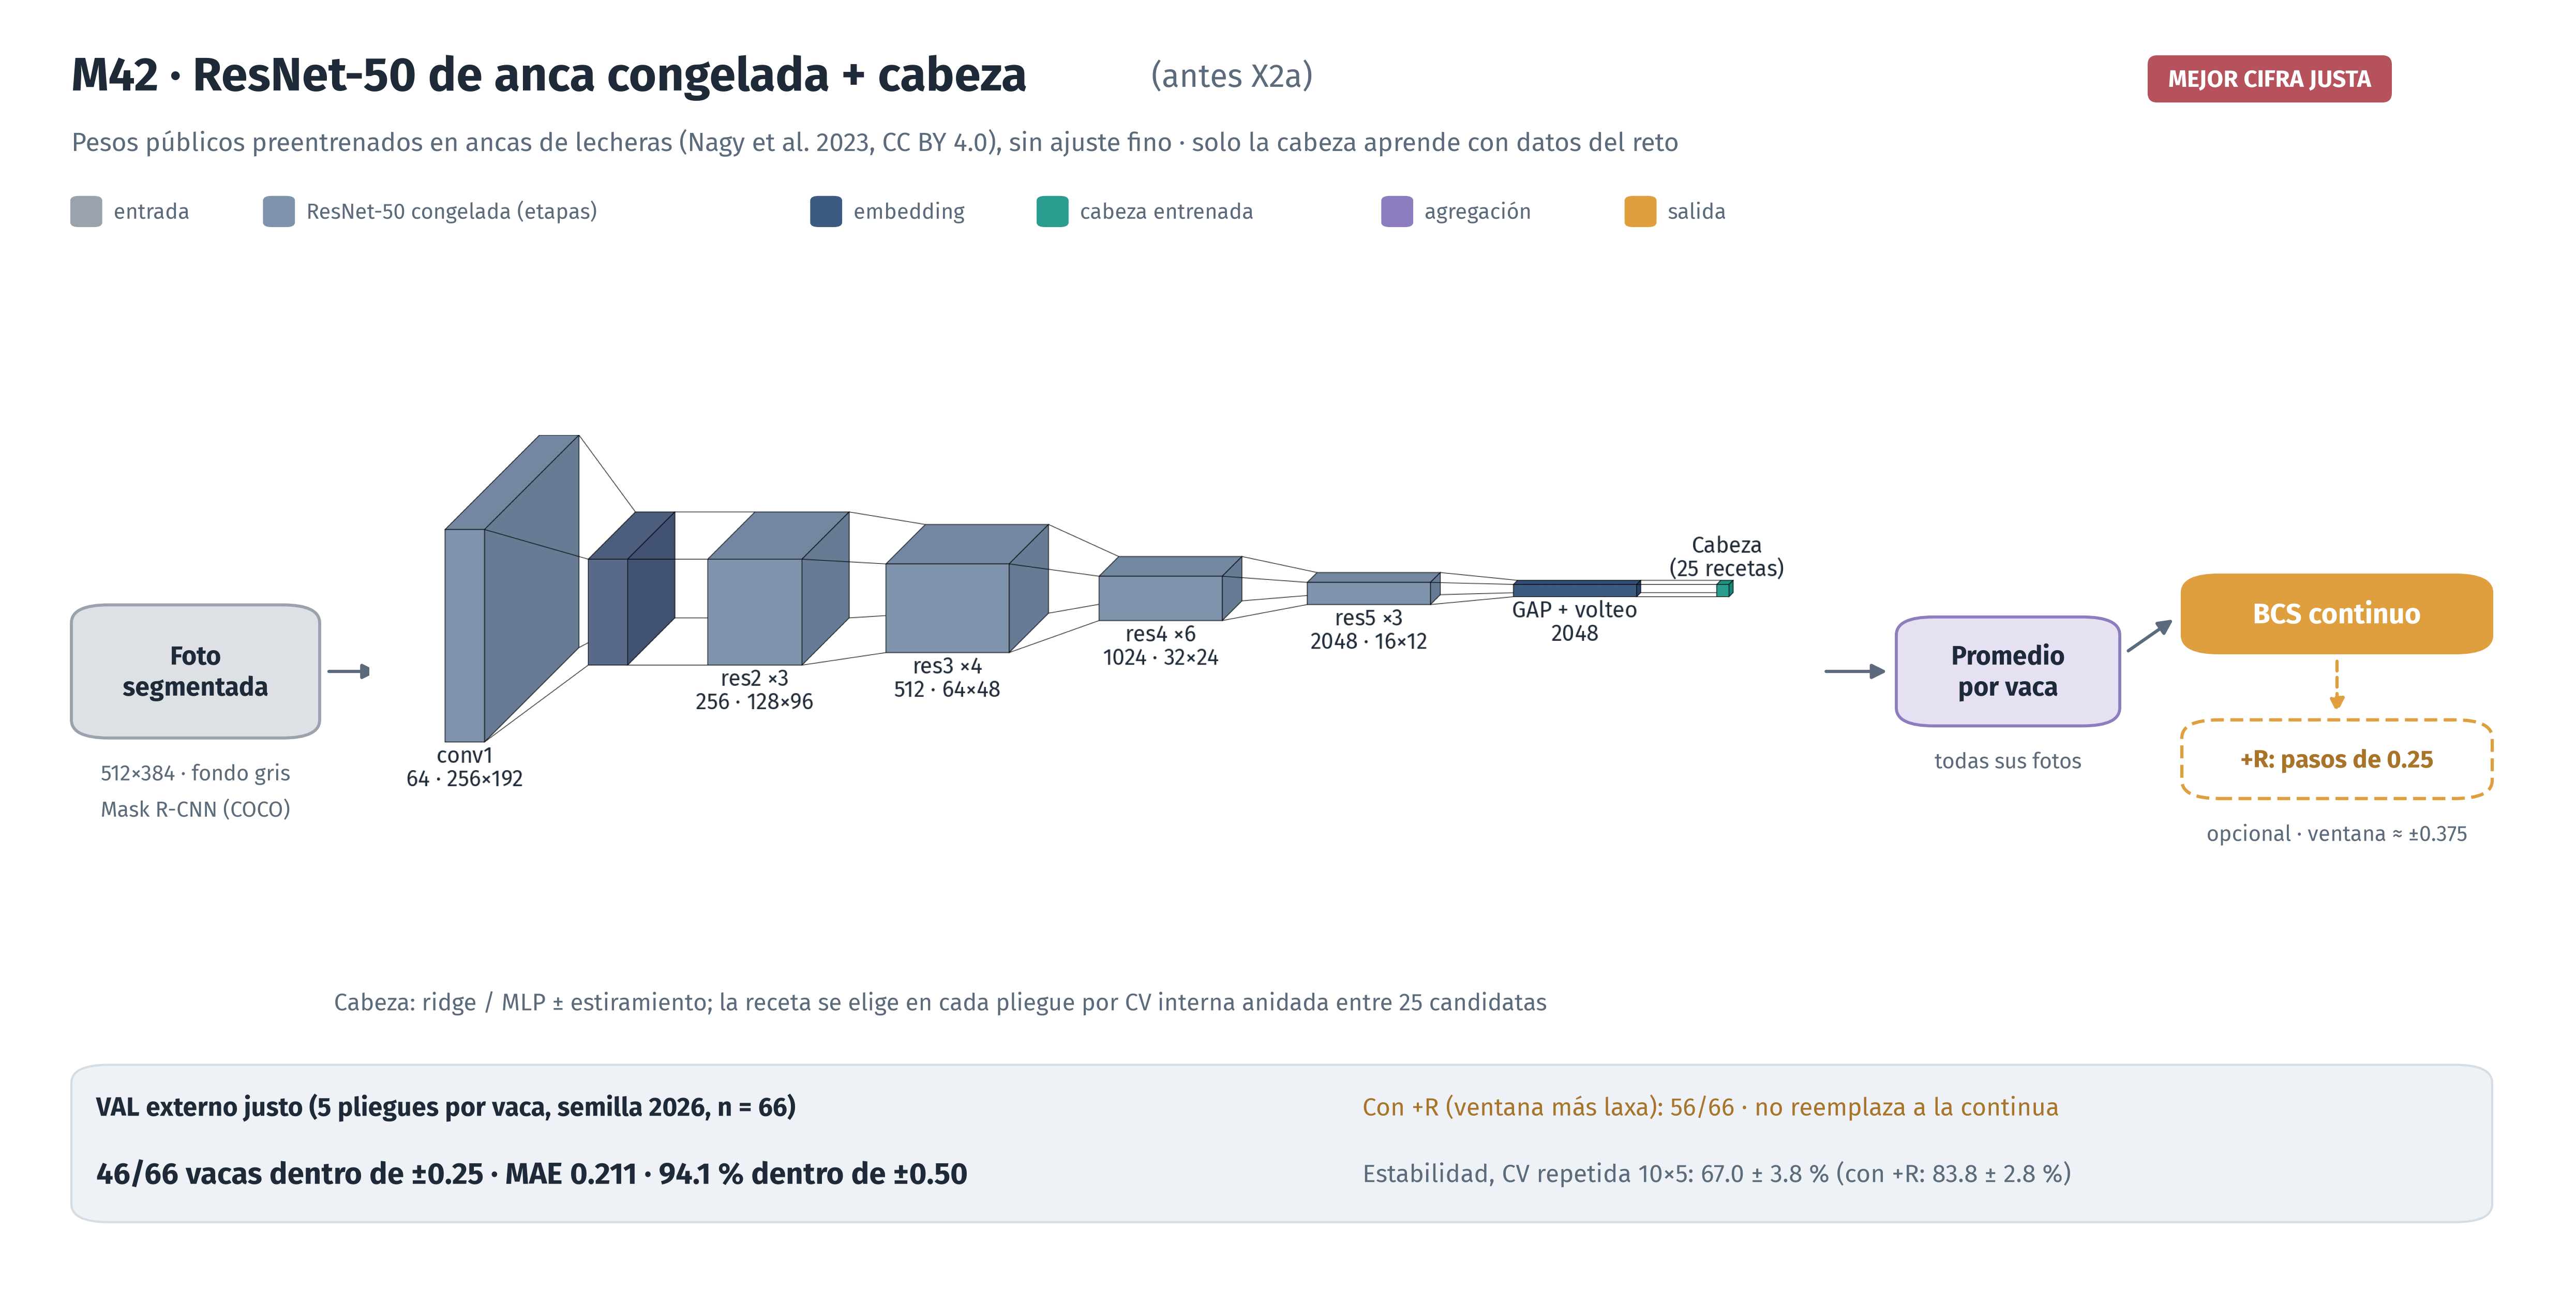
\includegraphics[width=\textwidth]{figures/modelo4}
  \caption{Arquitectura del Modelo 4 (ResNet-50 de vacas).}
  \label{fig:modelo4}
\end{figure}

\begin{figure}[H]
  \centering
  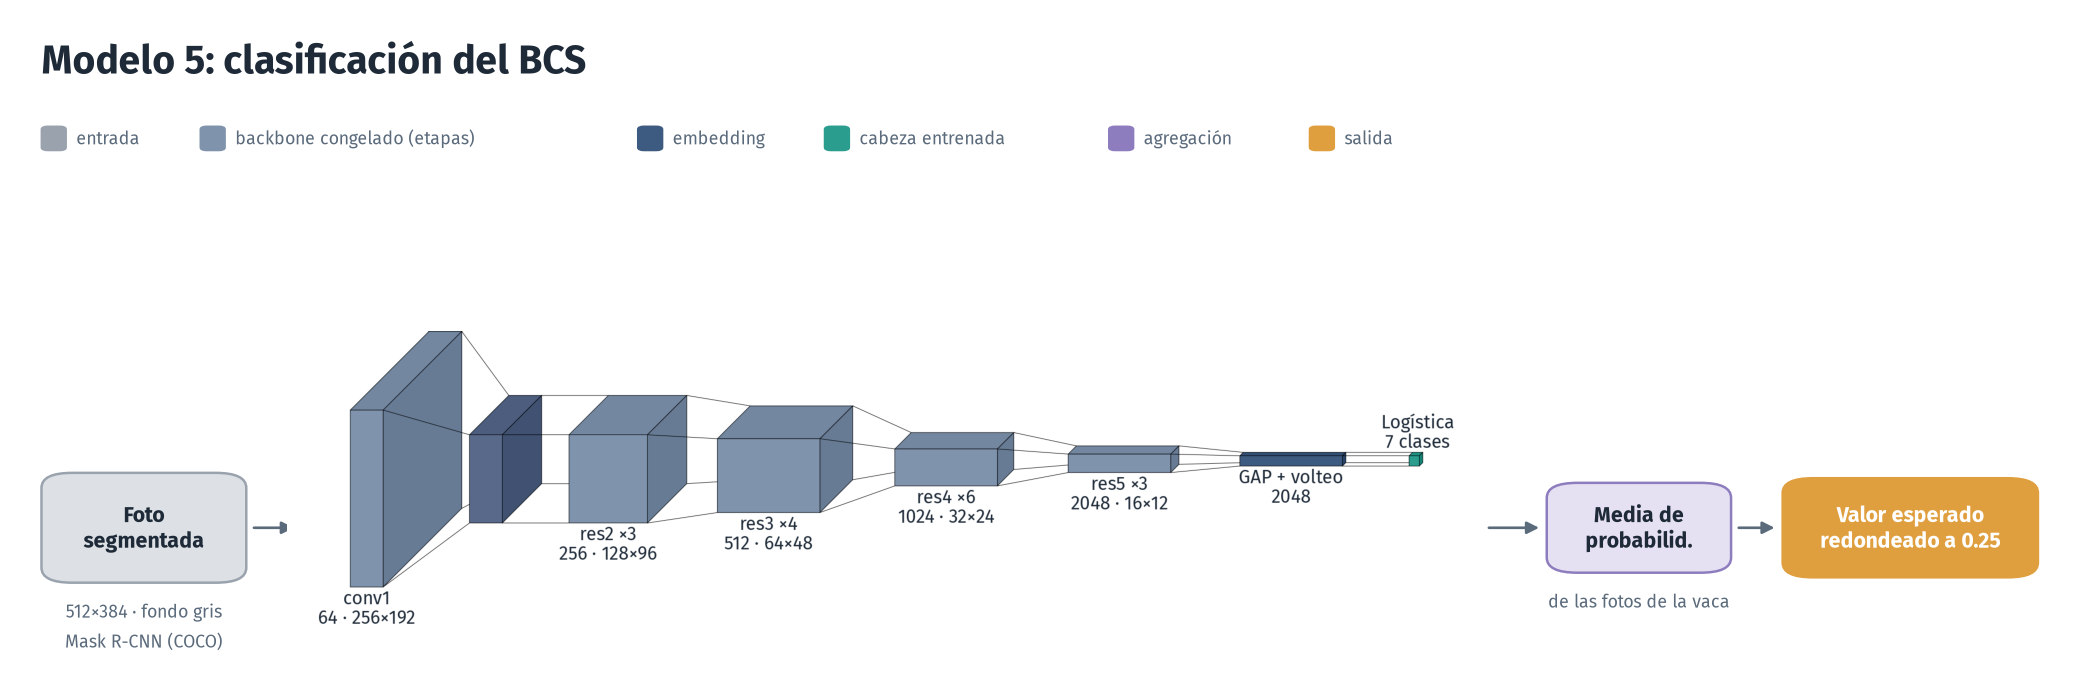
\includegraphics[width=\textwidth]{figures/modelo5}
  \caption{Arquitectura del Modelo 5 (clasificación del BCS).}
  \label{fig:modelo5}
\end{figure}
